% 旋度 斯托克斯定理
% 多元微积分|矢量场|散度|线积分|通量|环流量|旋度|斯托克斯定理

\pentry{圆周运动的速度\upref{CMVD}, 散度\upref{Divgnc}, 线积分\upref{IntL}, 流密度, 通量}%未完成
我们在矢量场中取一个闭合回路 $\mathcal L$ 并规定一个正方向, 并定义该回路的\textbf{环流量}为矢量场在回路上的线积分
\begin{equation}
\oint_{\mathcal L} \bvec F(\bvec r) \vdot \dd{\bvec r}
\end{equation}
下面我们来定义\textbf{旋度}, 旋度是一个矢量, 记为 $\curl \bvec F$. 在空间某点 $(x,y,z)$ 处选取一个小面元 $\bvec S$(模长为面元的面积, 方向为面元的一个法向量), 令面元边界构成的回路为 $\mathcal L$, 正方向由右手定则\upref{RHRul} 判断. 要定义其 $x$ 方向的分量, 就取 $\bvec S$ 与 $\uvec x$ 同向, 即
\begin{equation}
(\curl\bvec F)_x = \lim_{S\to 0} \frac 1S \oint_{\mathcal L} \bvec F(\bvec r) \vdot \dd{\bvec r}
\end{equation}
旋度的 $y, z$ 分量定义类似.

若矢量场分布连续且光滑, 则旋度处处存在且与回路的形状和坐标系的选取无关\footnote{本书不作证明}. 所以选取任意方向的面元 $\bvec S$, 都有
\begin{equation}\label{Curl_eq3}
\curl\bvec F \vdot \uvec S = \lim_{S\to 0} \frac 1S \oint_{\mathcal L} \bvec F(\bvec r) \vdot \dd{\bvec r}
\end{equation}

\subsection{直角坐标系中的旋度}
在直角坐标系中给出矢量场
\begin{equation}
\bvec F(x,y,z) = F_x(x,y,z)\uvec x + F_y(x,y,z)\uvec y + F_z(x,y,z)\uvec z
\end{equation}
在点 $(x,y,z)$ 附近, 我们可以对场使用微分近似
\begin{equation}
F_i(x+x', y+y', z+z') = F_i(x,y,z) + \pdv{F_i}{x}x' + \pdv{F_i}{y}y' + \pdv{F_i}{z}z'
\end{equation}

\begin{figure}[ht]
\centering
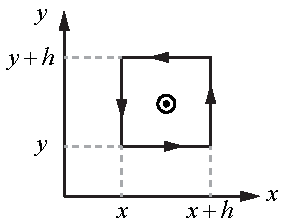
\includegraphics[width=5cm]{./figures/Curl1.pdf}
\caption{直角坐标系中旋度的 $z$ 分量} \label{Curl_fig1}
\end{figure}

要求 $z$ 方向的旋度, 令闭合回路为正方形 $[x,y,z]$-$[x+h, y+h, z]$(\autoref{Curl_fig1}), 延 $x$ 方向的两条边的线积分仅由 $F_x$ 贡献, 延 $y$ 方向的两条边的线积分仅由 $F_y$ 贡献, 所以整个环路的线积分为
\begin{equation}\ali{
\oint_{\mathcal L} \bvec F \vdot \dd{\bvec r}
&= \int_0^h \qty(F_x + \pdv{F_x}{x}x') \dd{x'} - \int_0^h \qty(F_x + \pdv{F_x}{x}x' + \pdv{F_x}{y}h) \dd{x'}\\
&\quad +\int_0^h \qty(F_y + \pdv{F_y}{x}h + \pdv{F_y}{y}y')\dd{y'} - \int_0^h  \qty(F_y + \pdv{F_y}{y}y') \dd{y'}\\
&= h^2 \qty(\pdv{F_y}{x} - \pdv{F_x}{y})
}\end{equation}
所以旋度的 $z$ 分量为
\begin{equation}\label{Curl_eq7}
G_z = \lim_{h^2\to 0} \frac{1}{h^2} \oint_{\mathcal L} \bvec F \vdot \dd{\bvec r} = \pdv{F_y}{x} - \pdv{F_x}{y}
\end{equation}
类似地, 我们可得 $x, y$ 分量
\begin{equation}
G_x = \pdv{F_z}{y} - \pdv{F_y}{z} \qquad G_y = \pdv{F_x}{z} - \pdv{F_z}{x}
\end{equation}
所以类似叉乘的行列式表示(\autoref{Cross_eq13}\upref{Cross}), 我们可以将旋度记为
\begin{equation}\label{Curl_eq9}
\curl \bvec F = \vmat{\uvec x & \uvec y & \uvec z\\ \pdv*{x}&\pdv*{y}&\pdv*{z}\\ F_x&F_y&F_z}
\end{equation}
现在我们知道为什么旋度要记为 $\curl \bvec F$ 了, 类比散度, 旋度可以从形式上理解为矢量算符 $\grad$ 与矢量场 $\bvec F$ 的叉乘.

与梯度和散度不同的是, 以上定义的旋度运算只能对三维空间的矢量场作用.

\begin{example}{旋转体速度场的旋度}
一个物体绕 $z$ 轴旋转, 角速度矢量为 $\bvec\omega = \omega\uvec z$, 物体上任意一点的位矢为 $\bvec r$, 则速度关于位置的函数 $\bvec v(\bvec r)$ 构成一个矢量场(\autoref{CMVD_eq5}\upref{CMVD}) 
\begin{equation}
\bvec v(\bvec r) = \bvec\omega \cross \bvec r = \omega\uvec z \cross (x\uvec x + y\uvec y)
= -\omega y\uvec x + \omega x\uvec y
\end{equation}
使用\autoref{Curl_eq9} 计算 $\bvec v(\bvec r)$ 的散度, 得
\begin{equation}
\curl \bvec v = \vmat{\uvec x&\uvec y&\uvec z\\ \pdv*{x}&\pdv*{y}&\pdv*{z}\\-\omega y&\omega x& 0} = 2\omega \uvec z
\end{equation}
可见该场的旋度是一个 $\uvec \omega$ 方向的常矢量. 从这个例子也可以看出, 如果一个(三维)矢量场在某个方向没有分量(即平面场), 则其旋度必然延该方向(即平面的法向量).
\end{example}

\begin{example}{无旋度的旋转场}
现在我们来看另一个旋转场 $\bvec F(\bvec r) = \uvec z\cross\uvec r /r$, 写成分量的形式就是
\begin{equation}
\bvec F(\bvec r) = \uvec z \cross \qty(\frac{x}{x^2 + y^2}\uvec x + \frac{y}{x^2 + y^2}\uvec y) = -\frac{y}{x^2 + y^2} \uvec x + \frac{x}{x^2 + y^2}\uvec y
\end{equation}
由于这个场也是一个 $xy$ 平面场, 旋度 $\uvec z$ 共线, 可以直接使用\autoref{Curl_eq7} 计算
\begin{equation}
\curl\bvec F = \qty(\pdv{F_y}{x} - \pdv{F_x}{y})\uvec z = \qty(\frac{1}{r^2} - \frac{2x^2}{r^4} + \frac{1}{r^2} - \frac{2y^2}{r^4})\uvec z = \bvec 0
\end{equation}
要注意的是, 在原点处由于矢量场不连续(而是出现了无限大的奇点), 以上计算在原点处并不成立. 
% 未完成:以后会在XXX详细讨论原点处的旋度如何表示.
\end{example}

\subsection{斯托克斯定理}

\begin{figure}[ht]
\centering
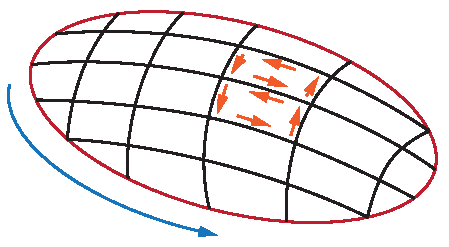
\includegraphics[width=6cm]{./figures/Curl2.pdf}
\caption{斯托克斯定理} \label{Curl_fig2}
\end{figure}

如\autoref{Curl_fig2}, 我们选取一块曲面, 并规定一个正方向. 使用右手定则\upref{RHRul}, 我们也可以定义曲面边界的正方向. 空间中存在连续光滑的矢量场 $\bvec F(\bvec r)$, 则\textbf{斯托克斯定理}可以将矢量场在曲面边界上的环流量和矢量场的旋度在曲面上通量等同起来
\begin{equation}
\oint \bvec F(\bvec r) \vdot \dd{\bvec r} = \iint \curl \bvec F(\bvec r) \vdot \dd{\bvec s}
\end{equation}


要证明这个定理, 我们将曲面划分为许多小面元 $\Delta \bvec s_i$, 其正方向与曲面一致, 边界的正方向同样由右手定则定义. 这样, 矢量场在曲面上的通量就等于在每个小面元上的通量之和. 当面元的面积趋于零时, 我们可以认为场的旋度在面元上是常矢量 $\bvec F(\bvec r_i)$, $\bvec r_i$ 为 $\Delta \bvec s_i$ 上任意一点. 由\autoref{Curl_eq3} 可知面元的环流量为 $\curl\bvec F(\bvec r_i) \vdot \Delta \bvec s_i$(可类比\autoref{Diff_eq2}\upref{Diff}), 所以根据积分的思想, 所有面元的环流量之和为
\begin{equation}
\lim_{\Delta s_i \to 0}\sum_i \curl\bvec F(\bvec r_i) \vdot \Delta \bvec s_i = \iint \curl\bvec F(\bvec r) \vdot \dd{\bvec s}
\end{equation}
最后, 如何证明所有面元的环流量之和等于曲面边界的环流量呢? 类比散度定理(\autoref{Divgnc_eq13}\upref{Divgnc})的证明, 考虑任意两块相邻的小面元, 矢量场在它们共同边界的线积分对一个面元的环流量贡献为正, 而对另一个面元的环流量贡献大小相同但符号为负, 所以在上式的求和中相加为零. 所以, 求和中唯一没有被抵消的环流量来自于曲面边界处的面元, 这些面元的边界与曲面边界重合且正方向一致, 对求和的贡献恰好等于曲面边界的环流量. 证毕.
